\documentclass[journal]{IEEEtran}
\IEEEoverridecommandlockouts

\usepackage{cite}
\usepackage{amsmath,amssymb,amsfonts}
\usepackage{algorithm}
\usepackage{algorithmic}
\usepackage{graphicx}
\usepackage{textcomp}
\usepackage{xcolor}
\usepackage{booktabs}
\usepackage{placeins}
\usepackage{multirow}
\usepackage{siunitx}
\usepackage{pgfplots}
\usepackage{tikz}
\usetikzlibrary{arrows.meta,positioning,shapes.geometric,calc,fit,backgrounds}
\pgfplotsset{compat=1.18}
\usepackage[hidelinks]{hyperref}
\hypersetup{pdftitle={LLM-Guard: A Calibrated Three-Layer Cascade for Prompt-Level Harm Detection, and What a Preregistered Test Set Says About It},pdfauthor={Omar Albulayhi and Muhammad Asif Habib}}

\sisetup{detect-weight=true,detect-family=true}

\definecolor{cAccent}{HTML}{2563EB}
\definecolor{cGood}{HTML}{16A34A}
\definecolor{cWarn}{HTML}{D97706}
\definecolor{cBad}{HTML}{DC2626}
\definecolor{cSlate}{HTML}{475569}
\definecolor{cPurple}{HTML}{7C3AED}
\definecolor{cTeal}{HTML}{0D9488}
\definecolor{cLight}{HTML}{F1F5F9}

\newcommand{\best}[1]{\textbf{#1}}
\newcommand{\posthoc}{\textsuperscript{\dag}}

\renewcommand{\topfraction}{0.92}
\renewcommand{\bottomfraction}{0.75}
\renewcommand{\textfraction}{0.06}
\renewcommand{\floatpagefraction}{0.80}
\renewcommand{\dbltopfraction}{0.92}
\renewcommand{\dblfloatpagefraction}{0.80}
\setcounter{topnumber}{3}
\setcounter{totalnumber}{4}
\setcounter{dbltopnumber}{3}

\usepackage{xr}
\externaldocument{main}
\externaldocument{supplementary_full}
\setcounter{table}{5}
\setcounter{figure}{2}
\setcounter{equation}{4}
\begin{document}
\title{Supplementary Material for ``LLM-Guard: A Calibrated Three-Layer Cascade for Prompt-Level Harm Detection, and What a Preregistered Test Set Says About It''}
\author{Omar~Albulayhi, Muhammad~Asif~Habib\\[2pt]
\parbox{\textwidth}{\centering\footnotesize \itshape Department of Computer Science\\
\itshape Imam Mohammad bin Saud Islamic University College of Computer and Information Sciences\\
\upshape Riyadh, Saudi Arabia\\
\upshape 446012900@sm.imamu.edu.sa, maabid@imamu.edu.sa}}
\maketitle

This is the supplementary material within the six pages the journal allows. The full version
is the file \texttt{docs/supplementary\_full.pdf} in the repository that accompanies the paper,
\url{https://github.com/OmarCSUF/LLM-Guard}. It adds the per-category rates of Table~VII and
the text of Sections S1--S26, which explains how each table and figure here was produced. Every
item keeps the same number in both versions, so the article's references hold for either.


\setcounter{figure}{2}
\begin{figure}[h]
\centering
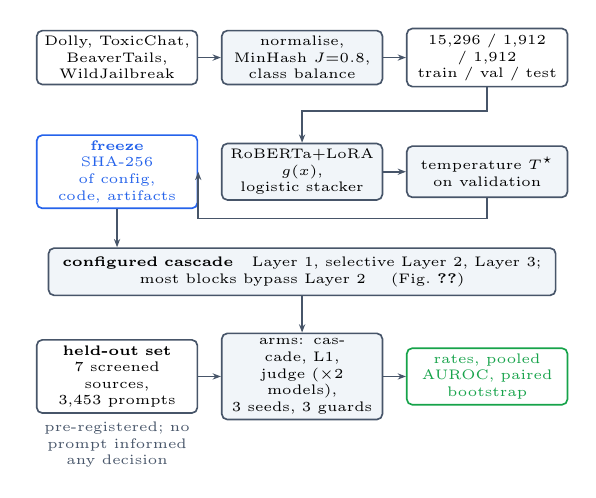
\begin{tikzpicture}[
  font=\tiny,
  box/.style={rounded corners=2pt,draw,semithick,align=center,inner sep=2pt,
              minimum height=6.5mm,text width=19mm},
  src/.style={box,fill=white,draw=cSlate},
  prc/.style={box,fill=cLight,draw=cSlate},
  frz/.style={box,fill=white,draw=cAccent,text=cAccent},
  inf/.style={box,fill=cLight,draw=cSlate,text width=63mm,minimum height=6mm},
  res/.style={box,fill=white,draw=cGood,text=cGood},
  ar/.style={-{Stealth[length=3pt]},draw=cSlate,semithick},
  bl/.style={font=\tiny,text=cSlate,inner sep=1pt}
]
\node[src] (corp) at (0,0)    {Dolly, ToxicChat,\\BeaverTails,\\WildJailbreak};
\node[prc] (scr)  at (2.35,0) {normalise,\\MinHash $J{=}0.8$,\\class balance};
\node[src] (spl)  at (4.70,0) {15{,}296 / 1{,}912\\/ 1{,}912\\train / val / test};
\draw[ar] (corp) -- (scr);
\draw[ar] (scr)  -- (spl);

\node[prc] (fit) at (2.35,-1.45) {RoBERTa+LoRA $g(x)$,\\logistic stacker};
\node[prc] (cal) at (4.70,-1.45) {temperature $T^\star$\\on validation};
\node[frz] (frz) at (0,-1.45)    {\textbf{freeze}\\SHA-256 of config,\\code, artifacts};
\draw[ar] (spl.south) -- ++(0,-0.30) -| (fit.north);
\draw[ar] (fit) -- (cal);
\draw[ar] (cal.south) -- ++(0,-0.26) -| (frz.east);

\node[inf] (casc) at (2.35,-2.72)
  {\textbf{configured cascade}\quad Layer 1, selective Layer 2, Layer 3;\\
   most blocks bypass Layer 2 \quad(Fig.~\ref{fig:arch})};
\draw[ar] (frz.south) -- (casc.north -| frz.south);

\node[src] (test) at (0,-4.05)    {\textbf{held-out set}\\7 screened sources,\\3{,}453 prompts};
\node[prc] (arms) at (2.35,-4.05) {arms: cascade, L1,\\judge ($\times$2 models),\\3 seeds, 3 guards};
\node[res] (met)  at (4.70,-4.05) {rates, pooled\\AUROC, paired\\bootstrap};
\draw[ar] (casc.south) -- ++(0,-0.40) -| (arms.north);
\draw[ar] (test) -- (arms);
\draw[ar] (arms) -- (met);
\node[bl,below=0.6mm of test,anchor=north,text width=22mm,align=center]
  {pre-registered; no prompt informed any decision};
\end{tikzpicture}
\caption{End-to-end workflow. The training pool is deduplicated and split; the
detector and its calibration are fitted on it; the configuration is then frozen
by hash \emph{before} the held-out set is scored. Every arm scores identical
prompts. The freeze covers the cascade's own configuration, code and artifacts;
the external-guard arms are pinned by model revision instead. The shaded
inference block is expanded in Fig.~\ref{fig:arch}.}
\label{abr:fig:overview}
\end{figure}

\setcounter{algorithm}{0}
\begin{algorithm}[h]
\caption{Layer-1 detection with input views}
\label{abr:alg:l1}
\begin{algorithmic}[1]
\REQUIRE prompt $x$; stacker $F$; scaler $T^\star$; thresholds
         $\tau_{\mathrm{low}},\tau_{\mathrm{high}}$; flags \textsc{norm}, \textsc{views}
\ENSURE routed score $s^\star$ and decision $d$
\IF{$x$ is empty}
  \RETURN $(0.5,\ \textsc{gray zone})$
\ENDIF
\STATE $s^\star \leftarrow \textsc{Score}(x)$
\STATE $\mathcal{F} \leftarrow \emptyset$
\IF{\textsc{norm}}
  \STATE $(x_{\mathrm{rec}},A) \leftarrow \textsc{Normalise}(x)$
  \IF{$A \neq \emptyset$}
    \STATE $\mathcal{F} \leftarrow \mathcal{F} \cup \{x_{\mathrm{rec}}\}$
  \ENDIF
  \STATE $\mathcal{F} \leftarrow \mathcal{F} \cup \textsc{Payloads}(x)$
         \COMMENT{each decoded blob alone}
\ENDIF
\IF{\textsc{views}}
  \STATE $\mathcal{F} \leftarrow \mathcal{F} \cup \textsc{ClauseViews}(x)$
\ENDIF
\FORALL{$x' \in \mathcal{F}$}
  \STATE $s^\star \leftarrow \max\bigl(s^\star,\ \textsc{Score}(x')\bigr)$
         \COMMENT{maximum only; cannot decrease}
\ENDFOR
\IF{$s^\star < \tau_{\mathrm{low}}$}
  \STATE $d \leftarrow \textsc{allow}$
\ELSIF{$s^\star > \tau_{\mathrm{high}}$}
  \STATE $d \leftarrow \textsc{mitigate}$
\ELSE
  \STATE $d \leftarrow \textsc{gray zone}$
\ENDIF
\RETURN $(s^\star,\ d)$
\STATE \rule{\linewidth}{0.3pt}
\STATE \textbf{procedure} \textsc{Score}$(t)$
\IF{$F$ reads the scoring-LM features}
  \STATE $f_{\mathrm{curv}} \leftarrow \textsc{Curvature}(t)$;\ \
         $f_{\mathrm{rank}} \leftarrow \textsc{LogRank}(t)$
\ELSE
  \STATE $f_{\mathrm{curv}},f_{\mathrm{rank}} \leftarrow 0.5,\,0.5$
         \COMMENT{skipped, not computed}
\ENDIF
\STATE $g \leftarrow \textsc{Classifier}(t)$ \COMMENT{$P(\mathrm{allow}\mid t)$}
\STATE $s_{\mathrm{raw}} \leftarrow
        1 - F.P_{\mathrm{allow}}(f_{\mathrm{curv}},f_{\mathrm{rank}},g)$
\RETURN $\sigma\bigl(\mathrm{logit}(s_{\mathrm{raw}})/T^\star\bigr)$
\end{algorithmic}
\end{algorithm}

\setcounter{algorithm}{1}
\begin{algorithm}[h]
\caption{Layer-3 mitigation with the refusal veto}
\label{abr:alg:l3}
\begin{algorithmic}[1]
\REQUIRE prompt $x$; category $c$; severity $v$; escalation flag $e$;
         constraint engine $E$; Guard-LLM $Q$; refuse-always set $\mathcal{R}$
\ENSURE the mode actually served, and its output
\STATE $\mathrm{trig} \leftarrow E.\textsc{Categories}(x)$
\IF{$c \in \mathcal{R}$ \OR $\mathrm{trig} \cap \mathcal{R} \neq \emptyset$}
  \STATE $m \leftarrow \textsc{refuse}$
         \COMMENT{$\mathrm{trig}$ supplies the category the L1 route lacks}
\ELSIF{$v \geq 0.99$ \OR $e$}
  \STATE $m \leftarrow \textsc{refuse}$
\ELSE
  \STATE $m \leftarrow$ configured default, which is \textsc{refuse}
\ENDIF
\IF{$m \neq \textsc{safe-rewrite}$}
  \RETURN $\textsc{Serve}(m)$
\ENDIF
\STATE $\mathrm{declined} \leftarrow \textsc{false}$;\ \ $C \leftarrow \emptyset$
\FOR{$k = 1$ \TO $K'$}
  \STATE $y \leftarrow Q.\textsc{Generate}(x,\ \text{temperature}=0.7)$
  \IF{$y$ is the sentinel \textsc{refuse} \OR $y$ reads as a prose refusal}
    \STATE $\mathrm{declined} \leftarrow \textsc{true}$
    \STATE \textbf{if} refuse-on-decline \textbf{then break}
           \COMMENT{the refusal veto}
  \ELSE
    \STATE $C \leftarrow C \cup \bigl\{(\,|E.\textsc{Check}(y)|,\ y)\bigr\}$
  \ENDIF
\ENDFOR
\IF{$\mathrm{declined}$ \AND refuse-on-decline}
  \RETURN $\textsc{Serve}(\textsc{refuse})$
\ENDIF
\STATE sort $C$ by violation count, ascending
\IF{$C \neq \emptyset$ \AND $C[0]$ has zero violations}
  \RETURN $\textsc{Serve}(\textsc{safe-rewrite},\ C[0])$
\ENDIF
\RETURN $\textsc{Serve}(\textsc{refuse})$
\end{algorithmic}
\end{algorithm}

\setcounter{algorithm}{2}
\begin{algorithm}[h]
\caption{Cascade decision}
\label{abr:alg:cascade}
\begin{algorithmic}[1]
\REQUIRE prompt $x$; detector $D$; judge $J$ or $\bot$; mitigator $G$ or $\bot$
\ENSURE prediction $\hat{y}$, harm score $h$, escalation flag
\STATE $(s^\star,d) \leftarrow D.\textsc{Detect}(x)$
       \COMMENT{Algorithm~\ref{alg:l1}}
\IF{$d = \textsc{allow}$}
  \RETURN $(1,\ s^\star,\ \textsc{false})$
\ENDIF
\IF{$d = \textsc{mitigate}$}
  \STATE \textbf{if} $G \neq \bot$ \textbf{then} $G.\textsc{FromL1}(x,s^\star)$
  \RETURN $(0,\ s^\star,\ \textsc{false})$
\ENDIF
\IF{$J = \bot$}
  \RETURN $(1,\ s^\star,\ \textsc{false})$
         \COMMENT{unresolved band allows}
\ENDIF
\STATE $r \leftarrow J.\textsc{Judge}(x)$
\STATE $h \leftarrow \tfrac{1}{2}\bigl(s^\star + r.\mathrm{severity}\bigr)$
\IF{$r.\mathrm{escalated}$}
  \STATE \textbf{if} $G \neq \bot$ \textbf{then} $G.\textsc{FromL2}(x,r)$
  \RETURN $(0,\ h,\ \textsc{true})$ \COMMENT{uncertainty blocks}
\ENDIF
\IF{$r.\mathrm{decision} = \textsc{allow}$}
  \RETURN $(1,\ h,\ \textsc{false})$
\ENDIF
\STATE \textbf{if} $G \neq \bot$ \textbf{then} $G.\textsc{FromL2}(x,r)$
\RETURN $(0,\ h,\ \textsc{false})$
\end{algorithmic}
\end{algorithm}

\setcounter{table}{5}
\begin{table}[h]
\caption{Layer-1 stackers on the pool test split ($n=1912$, balanced). Identical
inputs; scores quantised as the router serves them.}
\label{abr:tab:l1}
\centering
\footnotesize
\begin{tabular}{@{}lcc@{}}
\toprule
 & Classifier-only & Three-signal \\
 & (configured) & (\texttt{fusion\_v2}) \\
\midrule
AUROC              & \best{0.9914} & 0.9892 \\
AUPRC              & 0.9868 & \best{0.9877} \\
FPR @ 95\% TPR     & 0.0220 & 0.0220 \\
Accuracy           & 0.9629 & 0.9629 \\
Referred to judge  & 15 & 15 \\
Temperature $T^\star$ & 1.1908 & 1.1891 \\
\bottomrule
\end{tabular}
\end{table}

\setcounter{figure}{3}
\begin{figure}[h]
\centering
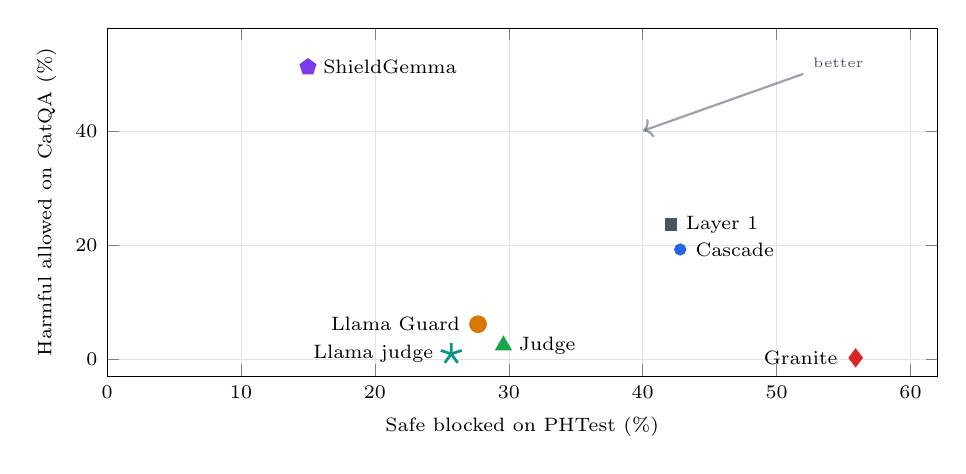
\begin{tikzpicture}
\begin{axis}[
  width=\columnwidth, height=6.0cm,
  xlabel={Safe blocked on PHTest (\%)},
  ylabel={Harmful allowed on CatQA (\%)},
  xmin=0,xmax=62,ymin=-3,ymax=58,
  grid=both, grid style={line width=.2pt,draw=gray!22},
  tick label style={font=\scriptsize}, label style={font=\scriptsize},
  every node near coord/.append style={font=\scriptsize},
  scatter/classes={
    a={mark=*,draw=cAccent,fill=cAccent},
    b={mark=square*,draw=cSlate,fill=cSlate},
    c={mark=triangle*,draw=cGood,fill=cGood,mark size=3.2pt},
    d={mark=diamond*,draw=cBad,fill=cBad,mark size=3.2pt},
    e={mark=pentagon*,draw=cPurple,fill=cPurple,mark size=3pt},
    f={mark=otimes*,draw=cWarn,fill=cWarn,mark size=3pt},
    g={mark=star,draw=cTeal,line width=1pt,mark size=4pt}},
]
\addplot[scatter,only marks,scatter src=explicit symbolic,
         nodes near coords*={\label},
         visualization depends on={value \thisrow{label} \as \label},
         every node near coord/.append style={anchor=west,xshift=2pt}]
table[meta=class] {
x     y     class label
42.8  19.2  a     {Cascade}
42.1  23.6  b     {Layer 1}
29.6  2.4   c     {Judge}
15.0  51.2  e     {ShieldGemma}
};
\addplot[scatter,only marks,scatter src=explicit symbolic,
         nodes near coords*={\label},
         visualization depends on={value \thisrow{label} \as \label},
         every node near coord/.append style={anchor=east,xshift=-3pt}]
table[meta=class] {
x     y     class label
27.7  6.1   f     {Llama Guard}
25.7  0.9   g     {Llama judge}
55.9  0.2   d     {Granite}
};
\draw[->,cSlate,thick,opacity=.55] (axis cs:52,50) -- (axis cs:40,40);
\node[font=\tiny,text=cSlate,anchor=west] at (axis cs:52,52) {better};
\end{axis}
\end{tikzpicture}
\caption{Operating points on PHTest and CatQA. Lower-left is better on
both axes at once. Llama Guard dominates the cascade here; Granite allows
less harm but blocks far more safe prompts, so at its own operating point it is
lower and to the \emph{right}, and dominates only at the matched threshold of
Table~\ref{tab:matched}. ShieldGemma occupies the opposite corner. Llama Guard's
advantage does not hold on Do-Not-Answer core, which this view does not show
(Table~\ref{tab:rates}). The star is the cascade's own Layer-2 slot holding
Llama-3.2-3B (Section~\ref{sec:judgeswap}): it dominates every arm here except
the two extremes, and is closest to the lower-left corner on either coordinate
taken together.}
\label{abr:fig:operating}
\end{figure}

\setcounter{figure}{4}
\begin{figure*}[h]
\centering
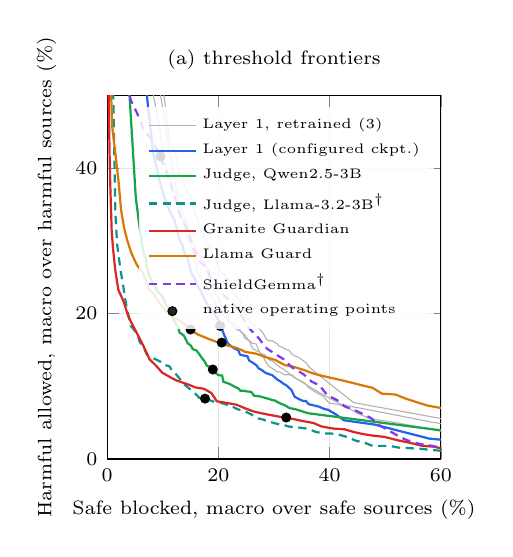
\begin{tikzpicture}
\begin{axis}[
  width=0.48\textwidth, height=6.2cm,
  xlabel={Safe blocked, macro over safe sources (\%)},
  ylabel={Harmful allowed, macro over harmful sources (\%)},
  xmin=0,xmax=60,ymin=0,ymax=50,
  grid=both, grid style={line width=.2pt,draw=gray!22},
  tick label style={font=\scriptsize}, label style={font=\scriptsize},
  legend style={font=\tiny,at={(0.98,0.97)},anchor=north east,draw=none,fill=white,fill opacity=0.85,text opacity=1},
  legend cell align=left, title={(a) threshold frontiers}, title style={font=\scriptsize},
]
\addplot[gray!60,thin,no markers,forget plot] coordinates {(0.0,100.0) (9.92,51.75) (11.21,44.01) (12.38,41.7) (12.91,39.43) (13.38,38.95) (13.68,38.11) (14.15,37.2) (14.51,36.54) (14.81,36.18) (15.23,35.63) (15.4,35.45) (15.46,34.66) (15.82,34.0) (15.99,33.4) (16.19,33.16) (16.46,32.5) (16.74,31.83) (16.91,31.1) (17.28,30.68) (17.55,30.33) (17.78,29.96) (17.91,29.36) (18.44,29.24) (18.77,28.69) (18.8,28.27) (19.31,27.82) (19.54,27.39) (19.86,26.85) (20.13,26.21) (20.5,25.67) (20.97,25.42) (21.36,25.0) (21.78,24.7) (22.0,23.7) (22.2,23.52) (22.61,22.82) (23.07,22.46) (23.44,22.16) (23.74,21.8) (24.06,21.5) (24.27,20.89) (24.59,20.23) (24.86,19.63) (25.27,19.27) (25.54,19.15) (25.84,18.73) (26.46,18.43) (26.87,18.07) (27.46,17.83) (28.09,17.25) (28.6,16.5) (29.06,16.25) (29.71,16.25) (30.28,15.96) (30.54,15.84) (30.87,15.53) (31.52,15.35) (32.18,15.05) (32.72,14.93) (33.24,14.39) (33.63,14.21) (34.41,13.98) (34.98,13.67) (35.91,13.14) (36.27,12.66) (37.52,11.87) (39.85,10.45) (44.32,7.75) (100.0,0.0)};
\addplot[gray!60,thin,no markers,forget plot] coordinates {(0.0,100.0) (9.41,50.98) (11.85,39.38) (12.73,35.85) (13.29,33.49) (14.02,32.19) (14.22,30.83) (14.59,30.34) (14.96,29.74) (15.16,29.2) (15.3,28.9) (15.65,27.87) (16.03,26.69) (16.15,25.96) (16.44,25.42) (16.77,25.0) (17.24,24.36) (17.77,23.99) (18.1,23.5) (18.4,22.96) (18.64,22.54) (18.94,22.0) (19.44,21.57) (19.67,21.09) (20.01,20.61) (20.33,20.24) (20.89,19.82) (21.31,19.57) (21.68,19.09) (22.05,18.79) (22.51,18.5) (22.85,18.2) (23.27,17.83) (23.93,17.59) (24.42,17.28) (24.89,16.92) (25.21,16.56) (25.6,16.2) (25.88,15.6) (26.27,15.12) (26.83,14.89) (27.39,14.71) (27.81,14.28) (28.2,13.86) (28.54,13.28) (29.05,12.77) (29.74,12.42) (30.04,12.29) (30.53,12.0) (31.15,11.94) (31.81,11.58) (32.61,11.58) (33.37,11.52) (33.87,11.11) (34.44,10.86) (35.16,10.62) (35.76,10.26) (36.08,9.9) (37.54,9.15) (37.97,8.97) (38.85,8.62) (39.88,7.7) (41.34,7.53) (43.19,7.1) (44.99,6.29) (47.3,5.53) (51.99,4.99) (58.16,4.09) (70.38,2.36) (100.0,0.0)};
\addplot[gray!60,thin,no markers] coordinates {(0.0,100.0) (5.27,64.58) (7.54,52.96) (8.88,47.87) (9.45,45.47) (9.98,42.18) (10.22,41.15) (10.99,39.1) (11.16,38.74) (11.46,38.25) (11.83,37.34) (12.12,36.86) (12.38,36.51) (12.59,36.21) (12.72,35.43) (13.07,34.83) (13.33,34.28) (13.71,33.74) (14.06,32.77) (14.45,32.35) (14.62,31.53) (14.82,31.11) (15.19,30.57) (15.35,29.92) (15.65,29.49) (15.95,28.89) (16.28,28.34) (16.75,27.93) (17.01,27.45) (17.44,27.03) (17.72,26.49) (17.96,26.0) (18.23,25.24) (18.36,24.12) (18.78,23.75) (19.18,23.45) (19.48,22.63) (19.92,22.27) (20.24,21.79) (20.6,21.15) (21.04,20.91) (21.3,20.07) (21.63,19.77) (21.95,19.28) (22.09,18.8) (22.78,18.68) (23.21,18.38) (23.77,18.14) (23.9,17.6) (24.41,17.24) (24.68,16.7) (25.24,16.4) (26.08,15.92) (26.84,15.8) (27.18,15.04) (27.59,14.51) (28.31,14.33) (28.61,14.03) (29.2,13.61) (29.88,13.37) (30.63,12.89) (31.02,12.65) (31.59,12.4) (32.45,11.92) (33.63,11.2) (34.99,10.6) (37.7,9.32) (42.11,7.49) (58.67,5.03) (100.0,0.0)};
\addlegendentry{Layer 1, retrained (3)}
\addplot[cAccent,thick,no markers] coordinates {(0.0,100.0) (8.27,42.13) (9.6,37.69) (10.73,35.06) (11.37,33.86) (11.91,33.13) (12.11,32.76) (12.41,32.07) (12.74,30.88) (13.1,30.04) (13.52,29.44) (13.81,28.5) (14.1,28.02) (14.45,27.66) (14.68,27.0) (14.88,26.28) (15.18,25.43) (15.58,25.07) (15.9,24.58) (16.13,24.05) (16.4,23.63) (16.92,23.02) (17.28,22.32) (17.61,21.9) (17.85,21.54) (18.01,21.05) (18.75,20.45) (19.18,20.15) (19.42,19.85) (19.68,19.55) (20.13,18.86) (20.32,18.25) (20.81,17.53) (21.07,16.99) (21.35,16.57) (21.65,15.93) (22.09,15.63) (22.73,15.27) (23.63,14.91) (23.86,14.37) (24.42,14.25) (25.22,14.13) (25.53,13.54) (26.06,13.3) (26.84,12.89) (27.21,12.47) (27.8,12.23) (28.31,11.93) (28.77,11.75) (29.7,11.51) (30.16,11.21) (30.61,10.91) (31.17,10.67) (31.54,10.43) (32.32,10.07) (33.15,9.47) (33.71,8.56) (34.41,8.26) (35.29,7.96) (35.75,7.96) (36.22,7.54) (37.5,7.3) (38.16,7.18) (39.0,6.88) (39.73,6.76) (41.13,6.13) (42.59,5.32) (48.08,4.73) (57.98,2.79) (100.0,0.0)};
\addlegendentry{Layer 1 (configured ckpt.)}
\addplot[cGood,thick,no markers] coordinates {(0.0,100.0) (5.16,35.93) (5.97,31.02) (6.65,27.93) (6.9,27.75) (7.19,26.27) (7.39,25.74) (7.49,25.26) (7.9,24.85) (8.17,24.1) (8.51,23.74) (8.8,23.45) (9.03,23.04) (9.45,22.74) (9.79,22.51) (10.16,22.04) (10.43,21.4) (10.75,21.05) (10.92,20.88) (11.15,20.47) (11.47,19.84) (11.81,19.42) (12.34,18.56) (12.76,18.16) (13.04,17.35) (13.33,17.23) (13.78,16.99) (14.24,16.31) (14.5,15.9) (15.03,15.61) (15.43,15.09) (16.07,14.92) (16.17,14.8) (16.56,14.44) (17.05,13.87) (17.49,13.46) (17.92,12.83) (18.5,12.65) (18.75,12.47) (19.21,12.05) (19.51,11.82) (19.98,11.53) (20.68,11.47) (20.91,10.61) (21.38,10.49) (21.65,10.43) (22.15,10.26) (22.6,10.08) (23.0,9.9) (23.54,9.73) (23.99,9.38) (24.72,9.38) (24.89,9.32) (25.48,9.26) (25.94,9.2) (26.43,8.69) (27.31,8.63) (27.92,8.51) (28.7,8.33) (29.06,8.27) (29.66,8.1) (30.16,8.04) (30.7,7.8) (31.17,7.62) (32.09,7.33) (32.67,7.04) (32.94,6.98) (34.0,6.81) (36.13,6.29) (100.0,0.0)};
\addlegendentry{Judge, Qwen2.5-3B}
\addplot[cTeal,thick,densely dashed,no markers] coordinates {(0.0,100.0) (1.47,34.05) (1.8,29.49) (2.41,26.0) (2.89,23.82) (3.19,22.32) (3.59,20.44) (3.95,19.5) (4.29,18.28) (4.99,17.63) (5.49,17.04) (5.86,16.1) (6.5,15.46) (7.19,14.3) (7.87,14.01) (8.71,13.71) (9.53,13.41) (10.24,12.94) (11.17,12.77) (11.75,12.07) (12.38,11.66) (12.95,11.14) (13.95,10.2) (14.7,9.73) (15.48,9.27) (16.09,8.8) (16.59,8.39) (17.45,8.33) (18.17,8.16) (18.98,7.92) (19.78,7.86) (20.89,7.63) (21.53,7.46) (22.29,7.34) (23.02,6.99) (23.79,6.76) (24.72,6.58) (25.47,6.29) (26.07,6.06) (27.1,5.59) (28.03,5.42) (28.93,5.18) (29.98,4.95) (31.13,4.72) (31.83,4.66) (32.56,4.48) (33.49,4.37) (34.55,4.31) (35.78,4.19) (36.73,3.96) (37.53,3.72) (38.25,3.61) (39.13,3.49) (40.35,3.49) (41.38,3.43) (42.31,3.2) (43.17,3.03) (44.18,2.68) (44.95,2.44) (45.88,2.44) (46.76,2.09) (47.74,1.8) (48.73,1.8) (50.02,1.8) (51.12,1.75) (52.84,1.51) (53.98,1.51) (56.25,1.4) (60.25,1.11) (100.0,0.0)};
\addlegendentry{Judge, Llama-3.2-3B$^\dag$}
\addplot[cBad,thick,no markers] coordinates {(0.0,71.94) (0.0,76.25) (0.0,80.59) (0.0,84.4) (0.0,88.25) (0.0,92.86) (0.0,97.1) (0.0,100.0) (0.09,65.27) (0.09,70.21) (0.18,60.59) (0.28,49.2) (0.28,53.2) (0.31,48.42) (0.43,42.58) (0.53,38.78) (0.62,36.38) (0.82,31.38) (1.04,29.13) (1.46,25.99) (2.02,23.27) (2.92,21.74) (3.85,19.52) (4.9,17.96) (5.83,16.61) (6.59,15.43) (7.64,13.69) (8.69,12.92) (9.89,11.88) (11.47,11.19) (12.53,10.78) (14.38,10.3) (15.91,9.83) (17.42,9.65) (18.74,9.07) (19.74,7.93) (21.63,7.69) (23.27,7.46) (24.73,6.99) (26.34,6.53) (27.74,6.29) (29.3,6.05) (31.36,5.76) (33.21,5.53) (35.41,5.18) (37.09,4.95) (38.51,4.48) (40.57,4.19) (42.67,4.08) (44.56,3.66) (46.43,3.37) (47.92,3.2) (49.91,3.03) (52.32,2.56) (54.53,2.21) (56.71,1.8) (58.73,1.69) (60.87,1.34) (63.42,1.16) (65.83,0.81) (68.53,0.58) (71.47,0.52) (74.16,0.41) (77.42,0.35) (80.99,0.23) (84.77,0.12) (88.82,0.06) (92.03,0.0) (96.08,0.0) (100.0,0.0)};
\addlegendentry{Granite Guardian}
\addplot[cWarn,thick,no markers] coordinates {(0.0,92.68) (0.0,98.13) (0.03,87.55) (0.03,92.31) (0.1,82.89) (0.17,65.8) (0.17,71.52) (0.17,75.82) (0.23,64.78) (0.51,57.4) (0.61,51.68) (0.7,50.7) (0.91,45.7) (1.23,43.65) (1.69,40.67) (2.05,38.2) (2.5,34.3) (3.07,31.71) (3.65,29.98) (4.41,28.22) (5.35,26.69) (6.45,25.55) (7.46,23.4) (8.31,22.75) (9.44,21.38) (10.6,20.37) (12.17,19.42) (13.68,18.71) (14.76,17.88) (16.42,17.08) (18.31,16.49) (20.2,15.95) (21.66,15.6) (23.39,15.25) (24.85,14.72) (26.73,14.49) (28.69,13.96) (30.27,13.6) (31.98,12.9) (33.58,12.67) (35.3,12.25) (37.15,11.73) (38.67,11.43) (40.33,11.14) (42.02,10.85) (44.3,10.43) (46.06,10.08) (47.71,9.79) (49.43,8.98) (51.85,8.86) (53.75,8.28) (55.91,7.75) (57.56,7.35) (59.74,7.05) (62.01,6.76) (64.12,6.46) (66.48,6.0) (68.27,5.53) (70.6,5.24) (73.04,4.95) (75.1,4.25) (77.25,3.9) (79.43,3.49) (81.88,2.91) (84.73,2.27) (87.38,1.86) (90.83,1.4) (93.25,0.87) (96.62,0.47) (100.0,0.0)};
\addlegendentry{Llama Guard}
\addplot[cPurple,thick,densely dashed,no markers] coordinates {(0.0,89.39) (0.0,94.85) (0.0,100.0) (0.19,82.71) (0.25,79.63) (0.46,75.63) (0.84,71.94) (1.03,69.42) (1.28,65.87) (1.96,61.18) (2.21,58.62) (2.98,55.25) (3.45,51.82) (4.28,49.3) (5.67,47.1) (6.48,45.45) (7.84,44.07) (9.08,42.42) (10.15,40.33) (11.26,38.24) (12.22,35.85) (13.16,33.34) (14.26,31.83) (15.08,29.95) (16.3,27.35) (17.87,26.38) (18.92,24.32) (20.08,23.24) (21.51,22.14) (23.25,20.85) (24.56,19.18) (25.6,17.92) (27.2,16.66) (28.71,15.19) (30.05,14.52) (31.67,13.75) (33.27,12.58) (35.28,11.67) (36.75,10.65) (38.19,10.11) (39.55,8.8) (41.36,8.09) (42.78,7.19) (44.38,6.76) (46.04,6.17) (47.42,5.64) (49.03,4.59) (50.17,4.11) (51.93,3.34) (53.4,2.75) (54.85,2.33) (56.36,2.04) (58.38,1.81) (60.53,1.45) (62.1,1.28) (63.88,1.22) (66.27,1.22) (68.11,1.11) (70.42,1.05) (72.56,0.93) (74.87,0.93) (77.72,0.81) (80.42,0.58) (82.2,0.47) (84.67,0.41) (87.63,0.17) (90.86,0.17) (93.11,0.0) (96.64,0.0) (100.0,0.0)};
\addlegendentry{ShieldGemma$^\dag$}
\addplot[only marks,mark=*,mark size=1.6pt,black] coordinates {(20.6,16.0) (20.3,18.3) (19.0,12.3) (17.6,8.3) (32.2,5.7) (15.0,17.8) (9.6,41.6)};
\addlegendentry{native operating points}
\end{axis}
\end{tikzpicture}\hfill
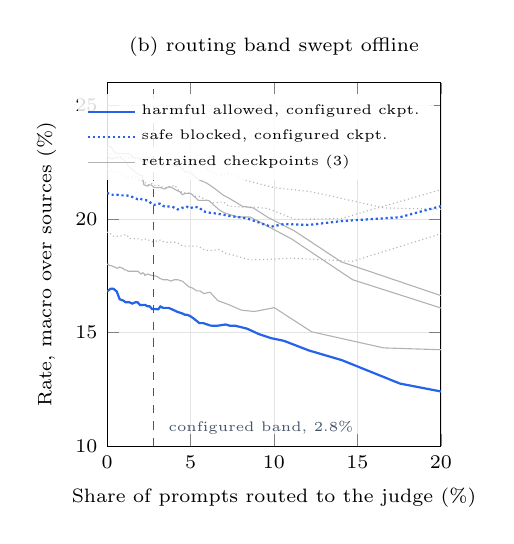
\begin{tikzpicture}
\begin{axis}[
  width=0.48\textwidth, height=6.2cm,
  xlabel={Share of prompts routed to the judge (\%)},
  ylabel={Rate, macro over sources (\%)},
  xmin=0,xmax=20,ymin=10,ymax=26,
  grid=both, grid style={line width=.2pt,draw=gray!22},
  tick label style={font=\scriptsize}, label style={font=\scriptsize},
  legend style={font=\tiny,at={(0.98,0.97)},anchor=north east,draw=none,fill=white,fill opacity=0.85,text opacity=1},
  legend cell align=left, title={(b) routing band swept offline}, title style={font=\scriptsize},
]
\addplot[gray!60,thin,no markers,forget plot] coordinates {(0.00,23.12) (0.14,23.18) (0.23,23.18) (0.38,23.00) (0.46,22.94) (0.67,22.88) (0.75,22.88) (0.84,22.88) (1.04,22.88) (1.10,22.88) (1.25,22.87) (1.30,22.87) (1.39,22.81) (1.48,22.81) (1.48,22.81) (1.59,22.69) (1.71,22.69) (1.85,22.69) (1.94,22.69) (2.09,22.57) (2.29,22.57) (2.37,22.51) (2.49,22.51) (2.69,22.51) (2.81,22.51) (3.04,22.38) (3.13,22.44) (3.24,22.38) (3.59,22.38) (3.65,22.38) (3.79,22.38) (4.05,22.32) (4.37,22.32) (4.58,22.14) (4.66,22.08) (4.95,22.07) (5.30,21.83) (5.56,21.71) (5.97,21.58) (6.34,21.40) (6.98,21.04) (7.30,20.92) (8.11,20.56) (8.75,20.49) (9.64,20.07) (11.24,19.47) (14.02,18.12) (61.92,6.19) (100.00,12.35) (100.00,12.35) (100.00,12.35)};
\addplot[gray!60,thin,densely dotted,no markers,forget plot] coordinates {(0.00,22.20) (0.14,22.20) (0.23,22.14) (0.38,22.10) (0.46,22.07) (0.67,22.04) (0.75,22.04) (0.84,22.00) (1.04,21.94) (1.10,21.85) (1.25,21.85) (1.30,21.85) (1.39,21.85) (1.48,21.85) (1.48,21.85) (1.59,21.85) (1.71,21.85) (1.85,21.78) (1.94,21.69) (2.09,21.69) (2.29,21.59) (2.37,21.59) (2.49,21.49) (2.69,21.56) (2.81,21.49) (3.04,21.46) (3.13,21.49) (3.24,21.42) (3.59,21.37) (3.65,21.37) (3.79,21.40) (4.05,21.49) (4.37,21.19) (4.58,21.19) (4.66,21.15) (4.95,21.15) (5.30,20.99) (5.56,20.99) (5.97,20.82) (6.34,20.72) (6.98,20.75) (7.30,20.56) (8.11,20.53) (8.75,20.53) (9.64,20.46) (11.24,19.99) (14.02,20.02) (61.92,30.20) (100.00,19.01) (100.00,19.01) (100.00,19.01)};
\addplot[gray!60,thin,no markers,forget plot] coordinates {(0.00,18.01) (0.09,18.01) (0.12,17.95) (0.26,17.95) (0.41,17.89) (0.46,17.89) (0.61,17.83) (0.75,17.89) (0.93,17.83) (0.96,17.83) (1.04,17.76) (1.13,17.76) (1.27,17.70) (1.36,17.70) (1.48,17.70) (1.62,17.70) (1.74,17.70) (1.85,17.70) (2.03,17.58) (2.14,17.64) (2.23,17.58) (2.26,17.52) (2.43,17.58) (2.66,17.52) (2.84,17.51) (3.04,17.45) (3.16,17.39) (3.36,17.33) (3.50,17.33) (3.62,17.33) (3.82,17.27) (4.03,17.33) (4.23,17.33) (4.52,17.26) (4.89,17.02) (5.13,16.96) (5.36,16.84) (5.56,16.84) (5.79,16.72) (6.17,16.78) (6.63,16.41) (7.30,16.23) (8.05,15.99) (8.83,15.93) (10.02,16.10) (12.25,15.04) (16.57,14.33) (100.00,12.35) (100.00,12.35) (100.00,12.35) (100.00,12.35)};
\addplot[gray!60,thin,densely dotted,no markers,forget plot] coordinates {(0.00,22.98) (0.09,22.88) (0.12,22.88) (0.26,22.88) (0.41,22.85) (0.46,22.81) (0.61,22.78) (0.75,22.75) (0.93,22.74) (0.96,22.74) (1.04,22.74) (1.13,22.74) (1.27,22.70) (1.36,22.64) (1.48,22.70) (1.62,22.67) (1.74,22.64) (1.85,22.64) (2.03,22.57) (2.14,22.50) (2.23,22.57) (2.26,22.57) (2.43,22.69) (2.66,22.66) (2.84,22.59) (3.04,22.59) (3.16,22.59) (3.36,22.56) (3.50,22.46) (3.62,22.46) (3.82,22.49) (4.03,22.42) (4.23,22.39) (4.52,22.36) (4.89,22.32) (5.13,22.32) (5.36,22.32) (5.56,22.36) (5.79,22.32) (6.17,22.10) (6.63,21.93) (7.30,22.02) (8.05,21.76) (8.83,21.60) (10.02,21.38) (12.25,21.20) (16.57,20.49) (100.00,19.01) (100.00,19.01) (100.00,19.01) (100.00,19.01)};
\addplot[gray!60,thin,no markers,forget plot] coordinates {(0.00,22.81) (0.14,22.69) (0.32,22.63) (0.38,22.69) (0.46,22.69) (0.64,22.69) (0.78,22.69) (0.98,22.63) (1.16,22.45) (1.27,22.33) (1.36,22.27) (1.53,22.14) (1.59,22.14) (1.68,22.09) (1.74,22.03) (1.91,21.96) (2.06,21.91) (2.09,21.91) (2.11,21.91) (2.20,21.51) (2.40,21.45) (2.55,21.50) (2.64,21.50) (2.75,21.44) (2.81,21.38) (3.07,21.38) (3.21,21.38) (3.42,21.32) (3.74,21.43) (3.91,21.37) (4.17,21.26) (4.37,21.19) (4.52,21.07) (4.69,21.13) (5.01,21.13) (5.21,21.00) (5.47,20.82) (5.82,20.82) (6.08,20.82) (6.72,20.40) (7.04,20.27) (7.82,20.09) (8.57,20.09) (9.53,19.72) (11.06,19.12) (14.71,17.33) (62.29,6.14) (64.06,6.49) (100.00,12.35) (100.00,12.35) (100.00,12.35)};
\addplot[gray!60,thin,densely dotted,no markers,forget plot] coordinates {(0.00,19.42) (0.14,19.42) (0.32,19.25) (0.38,19.25) (0.46,19.22) (0.64,19.25) (0.78,19.25) (0.98,19.28) (1.16,19.32) (1.27,19.22) (1.36,19.15) (1.53,19.15) (1.59,19.12) (1.68,19.15) (1.74,19.15) (1.91,19.12) (2.06,19.08) (2.09,19.08) (2.11,19.08) (2.20,19.12) (2.40,19.12) (2.55,19.05) (2.64,19.01) (2.75,19.01) (2.81,19.01) (3.07,19.05) (3.21,19.08) (3.42,18.98) (3.74,18.98) (3.91,18.98) (4.17,18.98) (4.37,18.88) (4.52,18.81) (4.69,18.81) (5.01,18.81) (5.21,18.81) (5.47,18.81) (5.82,18.65) (6.08,18.61) (6.72,18.65) (7.04,18.51) (7.82,18.36) (8.57,18.20) (9.53,18.22) (11.06,18.28) (14.71,18.14) (62.29,29.04) (64.06,28.74) (100.00,19.01) (100.00,19.01) (100.00,19.01)};
\addplot[cAccent,thick,no markers,forget plot] coordinates {(0.00,16.81) (0.20,16.93) (0.38,16.93) (0.58,16.81) (0.75,16.47) (0.98,16.41) (1.10,16.34) (1.16,16.34) (1.33,16.34) (1.51,16.28) (1.71,16.34) (1.82,16.34) (1.97,16.22) (2.06,16.22) (2.17,16.22) (2.26,16.22) (2.29,16.22) (2.40,16.16) (2.55,16.16) (2.69,16.04) (2.81,16.04) (3.07,16.03) (3.19,16.15) (3.36,16.09) (3.45,16.09) (3.68,16.09) (3.88,16.03) (4.23,15.91) (4.49,15.85) (4.66,15.79) (4.78,15.79) (4.98,15.73) (5.21,15.61) (5.53,15.42) (5.76,15.42) (6.20,15.31) (6.57,15.30) (7.10,15.36) (7.38,15.30) (7.70,15.30) (8.37,15.18) (9.09,14.94) (9.82,14.76) (10.60,14.64) (12.08,14.22) (14.07,13.79) (17.55,12.76) (61.54,6.53) (100.00,12.35) (100.00,12.35) (100.00,12.35)};
\addplot[cAccent,thick,densely dotted,no markers,forget plot] coordinates {(0.00,21.16) (0.20,21.07) (0.38,21.07) (0.58,21.07) (0.75,21.04) (0.98,21.04) (1.10,21.04) (1.16,21.04) (1.33,21.01) (1.51,20.97) (1.71,20.91) (1.82,20.87) (1.97,20.91) (2.06,20.87) (2.17,20.87) (2.26,20.84) (2.29,20.84) (2.40,20.81) (2.55,20.75) (2.69,20.65) (2.81,20.62) (3.07,20.67) (3.19,20.67) (3.36,20.58) (3.45,20.55) (3.68,20.55) (3.88,20.55) (4.23,20.42) (4.49,20.50) (4.66,20.50) (4.78,20.54) (4.98,20.47) (5.21,20.54) (5.53,20.50) (5.76,20.34) (6.20,20.27) (6.57,20.24) (7.10,20.17) (7.38,20.13) (7.70,20.10) (8.37,20.03) (9.09,19.85) (9.82,19.66) (10.60,19.78) (12.08,19.74) (14.07,19.91) (17.55,20.08) (61.54,28.83) (100.00,19.01) (100.00,19.01) (100.00,19.01)};
\addlegendimage{cAccent,thick}\addlegendentry{harmful allowed, configured ckpt.}
\addlegendimage{cAccent,thick,densely dotted}\addlegendentry{safe blocked, configured ckpt.}
\addlegendimage{gray!60,thin}\addlegendentry{retrained checkpoints (3)}
\draw[dashed,cSlate] (axis cs:2.8,10) -- (axis cs:2.8,26);
\node[font=\tiny,text=cSlate,anchor=west] at (axis cs:3.1,10.8) {configured band, 2.8\%};
\end{axis}
\end{tikzpicture}
\caption{Post hoc frontiers on the final test set, computed from stored
scores; no model was re-run. (a)~Each graded harm score with its threshold swept.
Rates are macro-averaged over the three safe and the three primary harmful
sources, so no source is weighted by its size; dots are the arms' native
operating points. Thresholds read off this set are descriptive, not matched
readings (Table~\ref{tab:matched}). (b)~The cascade's band $[0.5-w,\,0.5+w]$
swept in steps of $0.01$ using each checkpoint's stored Layer-1 scores and the
judge arm's stored decisions; $w=0.2$ is the configured band. Layer-1 scores
span $[0.034, 0.976]$, so the last steps of the sweep route
\SI{17.5}{\percent}, \SI{61.5}{\percent} and then every prompt, where the
cascade coincides with the judge-alone arm (19.0\% safe blocked, 12.3\%
harmful allowed); the axis is cut at \SI{20}{\percent}.}
\label{abr:fig:frontiers}
\end{figure*}

\setcounter{figure}{5}
\begin{figure}[h]
\centering
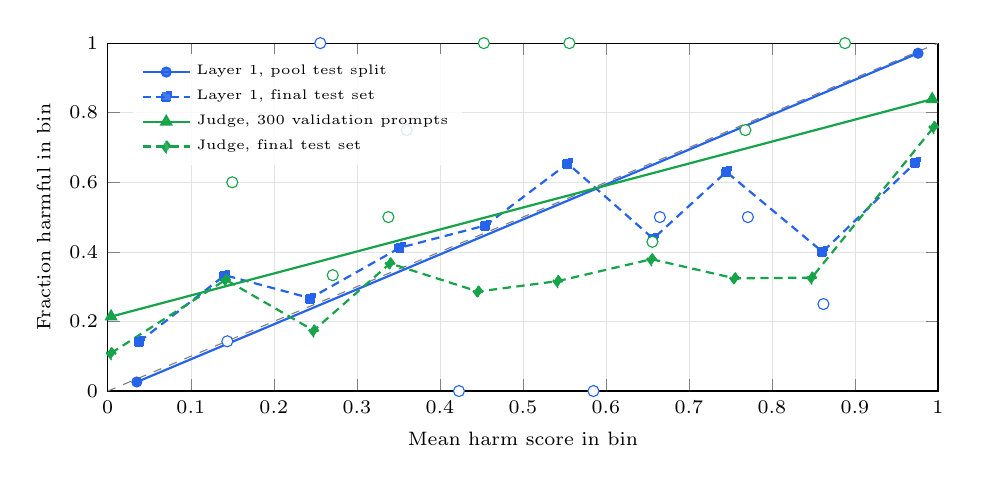
\begin{tikzpicture}
\begin{axis}[
  width=\columnwidth, height=6.0cm,
  xlabel={Mean harm score in bin}, ylabel={Fraction harmful in bin},
  xmin=0,xmax=1,ymin=0,ymax=1,
  grid=both, grid style={line width=.2pt,draw=gray!22},
  tick label style={font=\scriptsize}, label style={font=\scriptsize},
  legend style={font=\tiny,at={(0.03,0.97)},anchor=north west,draw=none,fill=white,fill opacity=0.85,text opacity=1},
  legend cell align=left,
]
\addplot[gray,dashed,no markers,forget plot] coordinates {(0,0) (1,1)};
\addplot[cAccent,thick,mark=*,mark size=1.6pt] coordinates {(0.035,0.026) (0.976,0.971)};
\addlegendentry{Layer 1, pool test split}
\addplot[cAccent,only marks,mark options={fill=white},forget plot] coordinates {(0.144,0.143) (0.256,1.000) (0.360,0.750) (0.423,0.000) (0.585,0.000) (0.665,0.500) (0.771,0.500) (0.862,0.250)};
\addplot[cAccent,thick,densely dashed,mark=square*,mark size=1.6pt] coordinates {(0.038,0.142) (0.141,0.333) (0.244,0.267) (0.352,0.412) (0.455,0.476) (0.554,0.654) (0.657,0.438) (0.745,0.630) (0.861,0.400) (0.973,0.657)};
\addlegendentry{Layer 1, final test set}
\addplot[cGood,thick,mark=triangle*,mark size=2pt] coordinates {(0.004,0.214) (0.993,0.839)};
\addlegendentry{Judge, 300 validation prompts}
\addplot[cGood,only marks,mark options={fill=white},forget plot] coordinates {(0.150,0.600) (0.271,0.333) (0.338,0.500) (0.453,1.000) (0.556,1.000) (0.656,0.429) (0.768,0.750) (0.888,1.000)};
\addplot[cGood,thick,densely dashed,mark=diamond*,mark size=2pt] coordinates {(0.004,0.109) (0.142,0.320) (0.248,0.174) (0.340,0.367) (0.446,0.286) (0.542,0.316) (0.655,0.379) (0.755,0.324) (0.848,0.326) (0.995,0.759)};
\addlegendentry{Judge, final test set}
\end{axis}
\end{tikzpicture}
\caption{Reliability of the Layer-1 score and the configured judge's
$p_{\mathrm{mit}}$, in distribution and on the final test set, in ten
equal-width bins; the diagonal is perfect calibration. Bins holding fewer than
ten prompts are drawn hollow and unconnected. Post hoc, from stored scores.
The two extreme bins hold almost all prompts: on the final test set
1{,}481 prompts score below 0.1 and 1{,}372 above 0.9 for Layer~1.}
\label{abr:fig:reliability}
\end{figure}

\setcounter{table}{7}
\begin{table}[h]
\caption{The configured judge under other decision bands and uncertain
policies, re-applied offline to its stored $p_{\mathrm{mit}}$ on the final test
set. Unc.\ is the share of prompts left uncertain; SB and HA are safe blocked
and harmful allowed, macro-averaged over sources, under the configured policy
(uncertain blocks) and the alternative (uncertain allows); the last two columns
are CoCoNot blocked and CatQA allowed under the configured policy. Percent;
post hoc; nothing was selected from this table.}
\label{abr:tab:judgeband}
\centering
\scriptsize
\setlength{\tabcolsep}{3pt}
\begin{tabular}{@{}lccccccc@{}}
\toprule
& & \multicolumn{2}{c}{Unc.\ blocks} & \multicolumn{2}{c}{Unc.\ allows} & & \\
\cmidrule(lr){3-4}\cmidrule(lr){5-6}
Band & Unc. & SB & HA & SB & HA & CoCoNot & CatQA \\
\midrule
$0.5$ threshold, no band & 0.0 & 18.0 & 12.8 & 18.0 & 12.8 & 19.3 & 3.1 \\
$0.45/0.55$ & 0.7 & 18.4 & 12.6 & 17.7 & 13.0 & 19.8 & 2.8 \\
$0.40/0.60$ (configured) & 1.4 & 19.0 & 12.3 & 17.5 & 13.5 & 20.4 & 2.4 \\
$0.30/0.70$ & 3.4 & 19.8 & 11.7 & 16.8 & 14.4 & 20.4 & 1.8 \\
$0.20/0.80$ & 5.4 & 20.7 & 11.5 & 15.6 & 15.0 & 21.2 & 1.8 \\
$0.05/0.95$ & 10.9 & 23.4 & 9.8 & 13.5 & 17.2 & 21.4 & 1.3 \\
\bottomrule
\end{tabular}
\end{table}

\setcounter{table}{8}
\begin{table}[h]
\caption{Component ablation on the final test set, configured checkpoint,
percent. View is the leading-clause view and $T=1$ replaces the fitted
temperature. To judge is the share of prompts routed to Layer~2; harmful sources
report harmful allowed and safe sources safe blocked; lower is better. Every
ablation arm is post hoc. Do-Not-Answer ``other'' is excluded as secondary.}
\label{abr:tab:ablation}
\centering
\scriptsize
\setlength{\tabcolsep}{2.5pt}
\begin{tabular}{@{}lcccccccc@{}}
\toprule
& To & Pooled & \multicolumn{3}{c}{Harmful allowed} & \multicolumn{3}{c}{Safe blocked} \\
\cmidrule(lr){4-6}\cmidrule(lr){7-9}
Arm & judge & AUROC & SST & CatQA & DNA & CoCoNot & PHTest & No Rob. \\
\midrule
Configured                 & 2.8 & 0.811 & 5.1 & 19.2 & 23.9 & 6.3 & 42.8 & 12.7 \\
View off\posthoc            & 2.8 & 0.814 & 5.1 & 19.2 & 23.9 & 6.3 & 42.6 & 11.7 \\
Normalisation off\posthoc  & 2.8 & 0.811 & 5.1 & 19.2 & 23.9 & 6.3 & 42.8 & 12.7 \\
Both off\posthoc           & 2.8 & 0.814 & 5.1 & 19.2 & 23.9 & 6.3 & 42.6 & 11.7 \\
$T=1$\posthoc               & 2.4 & 0.811 & 5.1 & 19.3 & 24.1 & 6.6 & 42.9 & 12.9 \\
\bottomrule
\end{tabular}
\end{table}

\setcounter{table}{9}
\begin{table}[h]
\caption{Routing-band alternatives on the pool validation split ($n=1912$,
balanced), classifier route, from the sweep recorded in the decision register.
This is selection data, not the final test set. To judge is the share routed
to Layer~2; the two rates are in percent.}
\label{abr:tab:sweep}
\centering
\footnotesize
\begin{tabular}{@{}lccc@{}}
\toprule
$\tau_{\mathrm{low}}$ / $\tau_{\mathrm{high}}$ & To judge & Safe blocked & Harmful allowed \\
\midrule
0.30 / 0.70 (configured) & 0.6 & 3.8 & 3.6 \\
0.50 / 0.50              & 0.0 & 3.7 & 3.5 \\
0.35 / 0.35              & 0.0 & 4.0 & 3.0 \\
0.05 / 0.50              & 1.9 & 4.6 & 2.9 \\
0.05 / 0.05              & 0.0 & 6.1 & 2.0 \\
0.00 / 0.05              & 48.0 & 18.5 & 1.1 \\
\bottomrule
\end{tabular}
\end{table}

\setcounter{table}{10}
\begin{table*}[!htbp]
\caption{Post hoc recalibration of the Layer-1 score and the judge's $p_{\mathrm{mit}}$. Columns 2--6: calibration error in distribution and on the final test set, Brier score and AUROC on the final test set. Columns 7--9: the configured $0.3/0.7$ band replayed on the recalibrated Layer-1 score, judge traffic as a percentage of primary prompts, macro safe blocked and macro harmful allowed.}
\label{abr:tab:calibalt}
\centering
\scriptsize
\setlength{\tabcolsep}{3pt}
\begin{tabular}{@{}lccccc ccc@{}}
\toprule
Calibrator & ECE val (fit) & ECE pool test & ECE final [95\% CI] & Brier & AUROC & Judge \% & SB & HA \\
\midrule
as served & 0.010 & 0.013 & 0.204 [0.191, 0.220] & 0.229 & 0.811 & 2.6 & 20.6 & 16.0 \\
temperature (refit) & 0.010 & 0.013 & 0.204 [0.190, 0.219] & 0.229 & 0.811 & 2.7 & 20.7 & 16.0 \\
Platt & 0.003 & 0.008 & 0.205 [0.190, 0.221] & 0.227 & 0.811 & 2.8 & 20.4 & 16.4 \\
isotonic & 0.000 & 0.008 & 0.143 [0.132, 0.159] & 0.199 & 0.810 & 17.9 & 18.0 & 14.4 \\
histogram binning & 0.000 & 0.004 & 0.200 [0.187, 0.216] & 0.227 & 0.766 & 4.9 & 19.3 & 16.4 \\
QaTS & 0.026 & 0.027 & 0.191 [0.177, 0.207] & 0.224 & 0.811 & 3.4 & 20.5 & 16.1 \\
multi-domain T (mean) & 0.019 & 0.027 & 0.186 [0.172, 0.203] & 0.222 & 0.811 & 3.1 & 20.6 & 16.2 \\
multi-domain T (worst-domain) & 0.091 & 0.095 & 0.112 [0.103, 0.130] & 0.200 & 0.811 & 4.8 & 20.5 & 15.7 \\
\midrule
Judge: as served & 0.191 & --- & 0.172 [0.159, 0.185] & 0.176 & 0.878 & & &  \\
Judge: temperature (refit) & 0.063 & --- & 0.078 [0.065, 0.091] & 0.136 & 0.878 & & &  \\
Judge: Platt & 0.029 & --- & 0.124 [0.111, 0.137] & 0.153 & 0.878 & & &  \\
Judge: isotonic & 0.000 & --- & 0.123 [0.112, 0.137] & 0.155 & 0.877 & & &  \\
Judge: histogram binning & 0.000 & --- & 0.118 [0.105, 0.133] & 0.168 & 0.811 & & &  \\
Judge: QaTS & 0.074 & --- & 0.068 [0.057, 0.082] & 0.136 & 0.878 & & &  \\
\bottomrule
\end{tabular}
\\[2pt]
\parbox{\linewidth}{\scriptsize Per-domain temperatures fitted on pool validation: BeaverTails 1.08, Dolly 0.99, ToxicChat 1.76, WildJailbreak 0.79. The averaged rule uses their mean; the worst-domain rule minimises the largest per-domain log loss. QaTS sets the temperature by the calibration-set quantile of the confidence. Histogram binning ties scores, so its AUROC falls.}
\end{table*}

\setcounter{table}{11}
\begin{table*}[!htbp]
\caption{Routing rules against the symmetric band at the same judge traffic. Band columns interpolate the symmetric band's curve to the rule's traffic; $\Delta$ is rule minus band in points, negative better.}
\label{abr:tab:routealt}
\centering
\scriptsize
\setlength{\tabcolsep}{3pt}
\begin{tabular}{@{}llccccccc@{}}
\toprule
Rule & Parameter & Judge \% & SB & HA & Band SB & Band HA & $\Delta$SB & $\Delta$HA \\
\midrule
high side 0.3/hi & 0.3/0.8 & 3.5 & 20.2 & 16.2 & 20.5 & 16.1 & -0.3 & +0.1 \\
high side 0.3/hi & 0.3/0.9 & 4.9 & 19.3 & 16.4 & 20.5 & 15.5 & -1.3 & +0.8 \\
high side 0.3/hi & 0.3/0.95 & 6.8 & 18.3 & 16.6 & 20.2 & 15.3 & -1.9 & +1.3 \\
high side 0.3/hi & 0.3/0.97 & 10.5 & 16.6 & 17.1 & 19.8 & 14.3 & -3.2 & +2.8 \\
high side 0.3/hi & 0.3/0.98 & 49.3 & 6.8 & 22.9 & 27.7 & 7.1 & -20.8 & +15.8 \\
low side lo/0.7 & 0.2/0.7 & 3.6 & 21.0 & 15.6 & 20.6 & 16.0 & +0.4 & -0.4 \\
low side lo/0.7 & 0.1/0.7 & 5.3 & 21.4 & 14.8 & 20.3 & 15.4 & +1.0 & -0.5 \\
low side lo/0.7 & 0.05/0.7 & 8.9 & 22.2 & 13.2 & 19.7 & 14.8 & +2.5 & -1.6 \\
low side lo/0.7 & 0.04/0.7 & 11.3 & 22.9 & 12.1 & 19.7 & 14.2 & +3.2 & -2.1 \\
isotonic score, symmetric band & 0.3/0.7 & 17.9 & 18.0 & 14.4 & 20.5 & 12.0 & -2.6 & +2.3 \\
isotonic score, symmetric band & 0.2/0.8 & 27.9 & 15.5 & 14.6 & 23.1 & 9.4 & -7.6 & +5.2 \\
isotonic score, symmetric band & 0.1/0.9 & 36.8 & 15.8 & 12.8 & 25.0 & 8.5 & -9.1 & +4.3 \\
isotonic score, symmetric band & 0.05/0.95 & 39.3 & 16.7 & 11.9 & 25.5 & 8.2 & -8.8 & +3.7 \\
worst-domain T, symmetric band & 0.3/0.7 & 4.8 & 20.5 & 15.7 & 20.5 & 15.7 & +0.0 & +0.0 \\
worst-domain T, symmetric band & 0.2/0.8 & 9.1 & 19.7 & 14.8 & 19.7 & 14.8 & -0.1 & +0.0 \\
checkpoint disagreement & spread > 0.6 & 17.4 & 18.4 & 14.1 & 20.5 & 12.4 & -2.1 & +1.7 \\
checkpoint disagreement & spread > 0.5 & 18.3 & 18.3 & 14.1 & 20.6 & 11.8 & -2.3 & +2.3 \\
checkpoint disagreement & spread > 0.3 & 19.6 & 18.1 & 14.2 & 20.7 & 11.1 & -2.7 & +3.1 \\
checkpoint disagreement & spread > 0.2 & 20.7 & 17.9 & 14.2 & 21.1 & 10.8 & -3.1 & +3.4 \\
checkpoint disagreement & spread > 0.1 & 22.6 & 18.2 & 14.0 & 21.6 & 10.4 & -3.4 & +3.6 \\
learned deferral & top 3\% & 2.6 & 20.0 & 16.9 & 20.7 & 16.0 & -0.6 & +0.9 \\
learned deferral & top 10\% & 9.1 & 19.4 & 15.2 & 19.7 & 14.8 & -0.3 & +0.5 \\
learned deferral & top 20\% & 18.9 & 18.3 & 14.0 & 20.6 & 11.4 & -2.3 & +2.6 \\
learned deferral & top 30\% & 28.9 & 16.7 & 12.6 & 23.3 & 9.3 & -6.5 & +3.3 \\
learned deferral & top 40\% & 40.0 & 14.0 & 14.0 & 25.7 & 8.1 & -11.7 & +5.8 \\
\bottomrule
\end{tabular}
\\[2pt]
\parbox{\linewidth}{\scriptsize Checkpoint disagreement routes a prompt when the largest and smallest Layer-1 scores of the four checkpoints differ by more than the threshold; the learned rule routes the stated share of prompts with the highest predicted chance that the judge corrects Layer~1.}
\end{table*}

\setcounter{table}{12}
\begin{table}[!htbp]
\caption{Conformal selective prediction: accept a decision when its confidence $\max(s,1-s)$ is at least $\lambda$, the smallest threshold giving error at most $\alpha$ among accepted validation prompts. Error and deferral in percent.}
\label{abr:tab:conformal}
\centering
\scriptsize
\setlength{\tabcolsep}{3pt}
\begin{tabular}{@{}lcccccc@{}}
\toprule
Score & $\alpha$ & $\lambda$ & Val err & Val defer & Final err & Final defer \\
\midrule
Layer 1 & 0.1 & 0.5199 & 3.6 & 0.0 & 25.2 & 0.3 \\
Layer 1 & 0.05 & 0.5199 & 3.6 & 0.0 & 25.2 & 0.3 \\
Layer 1 & 0.02 & 0.9654 & 2.0 & 6.9 & 21.8 & 24.8 \\
Layer 1 & 0.01 & 0.9763 & 0.9 & 54.9 & 28.1 & 73.8 \\
\midrule
Judge & 0.2 & 0.7154 & 19.9 & 4.3 & 18.3 & 3.7 \\
Judge & 0.15 & 0.9955 & 14.9 & 21.7 & 13.2 & 20.7 \\
Judge & 0.1 & 1.0000 & 9.1 & 67.0 & 8.8 & 39.2 \\
\bottomrule
\end{tabular}
\\[2pt]
\parbox{\linewidth}{\scriptsize No Layer-1 threshold on the final test set itself gives error at most 10\% among accepted prompts. At $\alpha=0.05$ no judge threshold meets the target on validation.}
\end{table}

\setcounter{table}{13}
\begin{table*}[!htbp]
\caption{Calibration error and Brier score of every graded arm on each primary source of the final test set (ECE / Brier). Each source is single-class, so a per-source error measures how far the scores sit from that class.}
\label{abr:tab:persource}
\centering
\scriptsize
\setlength{\tabcolsep}{3pt}
\begin{tabular}{@{}lccccccc@{}}
\toprule
Arm & SST & CatQA & DNA core & CoCoNot & PHTest & No Robots & Pooled \\
\midrule
Layer 1 & 0.079 / 0.051 & 0.228 / 0.181 & 0.249 / 0.209 & 0.101 / 0.061 & 0.444 / 0.401 & 0.164 / 0.119 & 0.204 / 0.229 \\
Layer 1 s42 & 0.098 / 0.070 & 0.370 / 0.324 & 0.267 / 0.232 & 0.082 / 0.047 & 0.474 / 0.435 & 0.175 / 0.132 & 0.252 / 0.270 \\
Layer 1 s43 & 0.099 / 0.066 & 0.256 / 0.207 & 0.251 / 0.211 & 0.090 / 0.055 & 0.475 / 0.428 & 0.181 / 0.138 & 0.226 / 0.245 \\
Layer 1 s44 & 0.083 / 0.054 & 0.380 / 0.328 & 0.247 / 0.210 & 0.092 / 0.046 & 0.440 / 0.393 & 0.150 / 0.101 & 0.222 / 0.247 \\
Judge & 0.030 / 0.020 & 0.031 / 0.023 & 0.334 / 0.312 & 0.196 / 0.188 & 0.285 / 0.255 & 0.065 / 0.050 & 0.172 / 0.176 \\
Llama judge & 0.003 / 0.001 & 0.013 / 0.008 & 0.259 / 0.220 & 0.211 / 0.190 & 0.259 / 0.191 & 0.061 / 0.038 & 0.129 / 0.133 \\
Granite & 0.017 / 0.002 & 0.015 / 0.003 & 0.180 / 0.116 & 0.236 / 0.159 & 0.547 / 0.386 & 0.240 / 0.135 & 0.211 / 0.188 \\
Llama Guard & 0.027 / 0.014 & 0.085 / 0.052 & 0.464 / 0.407 & 0.087 / 0.052 & 0.305 / 0.207 & 0.139 / 0.083 & 0.155 / 0.172 \\
ShieldGemma & 0.237 / 0.154 & 0.500 / 0.410 & 0.501 / 0.420 & 0.121 / 0.083 & 0.171 / 0.101 & 0.035 / 0.014 & 0.167 / 0.200 \\
\bottomrule
\end{tabular}
\end{table*}

\setcounter{table}{14}
\begin{table*}[!htbp]
\caption{AUROC of each harmful source against each safe source, harmful/safe: SimpleSafetyTests (SST), CatQA (CQ) and Do-Not-Answer core (DNA) against CoCoNot contrast (CC), PHTest (PH) and No Robots (NR).}
\label{abr:tab:pairwise}
\centering
\scriptsize
\setlength{\tabcolsep}{3pt}
\begin{tabular}{@{}lcccccccccccc@{}}
\toprule
Arm & Pooled & Mean & Min & SST/CC & SST/PH & SST/NR & CQ/CC & CQ/PH & CQ/NR & DNA/CC & DNA/PH & DNA/NR \\
\midrule
Cascade & 0.811 & 0.874 & 0.696 & 0.982 & 0.862 & 0.970 & 0.934 & 0.696 & 0.895 & 0.922 & 0.725 & 0.883 \\
Layer 1 & 0.811 & 0.874 & 0.695 & 0.982 & 0.861 & 0.970 & 0.934 & 0.695 & 0.894 & 0.922 & 0.725 & 0.883 \\
Judge & 0.878 & 0.905 & 0.749 & 0.923 & 0.947 & 0.994 & 0.933 & 0.957 & 0.994 & 0.791 & 0.749 & 0.856 \\
Llama judge & 0.928 & 0.951 & 0.823 & 0.977 & 0.993 & 1.000 & 0.977 & 0.988 & 0.998 & 0.871 & 0.823 & 0.929 \\
Granite & 0.923 & 0.950 & 0.801 & 0.988 & 0.979 & 0.994 & 0.990 & 0.982 & 0.994 & 0.911 & 0.801 & 0.913 \\
Llama Guard & 0.834 & 0.892 & 0.626 & 0.991 & 0.975 & 0.991 & 0.978 & 0.935 & 0.972 & 0.806 & 0.626 & 0.751 \\
ShieldGemma & 0.826 & 0.875 & 0.740 & 0.943 & 0.919 & 0.982 & 0.862 & 0.780 & 0.928 & 0.836 & 0.740 & 0.886 \\
\bottomrule
\end{tabular}
\end{table*}

\setcounter{table}{15}
\begin{table*}[!htbp]
\caption{4-bit against unquantised guards on the 599-prompt subset. AUROC difference is unquantised minus 4-bit with a paired bootstrap interval; agreement in percent; per-source rates at the matched threshold, 4-bit/unquantised, harmful allowed for SST, CatQA and DNA core and safe blocked for the rest.}
\label{abr:tab:quant}
\centering
\scriptsize
\setlength{\tabcolsep}{3pt}
\begin{tabular}{@{}lccccccccccc@{}}
\toprule
Guard & AUROC 4-bit & unquant. & $\Delta$ [95\% CI] & Native agr. & Matched agr. & SST & CatQA & DNA core & CoCoNot & PHTest & No Robots \\
\midrule
Granite Guardian & 0.9425 & 0.9430 & +0.0005 [-0.0042, +0.0054] & 93.2 & 92.5 & 12.1/19.2 & 9.0/19.0 & 41.0/58.0 & 2.0/1.0 & 10.0/2.0 & 3.0/1.0 \\
Llama Guard & 0.8872 & 0.8947 & +0.0075 [+0.0014, +0.0137] & 97.2 & 97.0 & 5.1/7.1 & 16.0/17.0 & 55.0/55.0 & 4.0/4.0 & 10.0/8.0 & 5.0/2.0 \\
ShieldGemma\posthoc & 0.8633 & 0.8663 & +0.0030 [-0.0001, +0.0064] & 98.5 & 98.3 & 29.3/30.3 & 59.0/61.0 & 52.0/54.0 & 9.0/9.0 & 10.0/6.0 & 1.0/0.0 \\
\bottomrule
\end{tabular}
\end{table*}

\setcounter{table}{16}
\begin{table*}[!htbp]
\caption{Harmful allowed on Do-Not-Answer core by risk area, percent with 95\% Wilson intervals.}
\label{abr:tab:riskarea}
\centering
\scriptsize
\setlength{\tabcolsep}{3pt}
\begin{tabular}{@{}lcccccccc@{}}
\toprule
Risk area & $n$ & Cascade & Layer 1 & Judge & Llama judge & Granite & Llama Guard & ShieldGemma \\
\midrule
discrimination & 175 & 17.1 [12.3, 23.4] & 17.1 [12.3, 23.4] & 26.3 [20.3, 33.3] & 14.9 [10.3, 20.9] & 4.6 [2.3, 8.8] & 66.3 [59.0, 72.9] & 19.4 [14.2, 25.9] \\
malicious & 243 & 13.6 [9.8, 18.5] & 16.0 [12.0, 21.2] & 2.5 [1.1, 5.3] & 3.3 [1.7, 6.4] & 0.0 [0.0, 1.6] & 15.2 [11.3, 20.3] & 44.4 [38.3, 50.7] \\
misinformation & 155 & 47.7 [40.0, 55.6] & 48.4 [40.7, 56.2] & 87.1 [80.9, 91.5] & 66.5 [58.7, 73.4] & 57.4 [49.5, 64.9] & 69.0 [61.4, 75.8] & 90.3 [84.6, 94.0] \\
\bottomrule
\end{tabular}
\end{table*}

\setcounter{table}{17}
\begin{table*}[!htbp]
\caption{Response classifiers on Layer~3 outputs. Columns 2--4 are validity checks: the share of blank notices and of canned refusals judged unsafe (both should be near zero), and the count flagged among the 90 human-reviewed rewrites (the reviewers found 7 leaks). Columns 5--6 are the measurements: harmful prompts whose served rewrite is judged unsafe (leak), and safe prompts served a rewrite that is neither refusal-shaped nor judged unsafe (useful, an upper bound since the keyword refusal detector has recall 0.34). Percent with Wilson 95\% intervals over the 60 prompts of each group.}
\label{abr:tab:mitigation}
\centering
\scriptsize
\setlength{\tabcolsep}{3pt}
\begin{tabular}{@{}lccccc@{}}
\toprule
Classifier & Blank flagged & Refusal flagged & Pilot 4 flagged & Leak, harmful & Useful, safe \\
\midrule
Llama Guard, request and response & 56.3 & 2.7 & 32/90 & 3.3 [0.9, 11.4] & 78.3 [66.4, 86.9] \\
Granite Guardian, request and response & 90.8 & 97.3 & 51/90 & 15.0 [8.1, 26.1] & 86.7 [75.8, 93.1] \\
Llama Guard, response alone & 99.2 & 0.0 & 17/90 & 1.7 [0.3, 8.9] & 78.3 [66.4, 86.9] \\
\bottomrule
\end{tabular}
\end{table*}

\setcounter{table}{18}
\begin{table*}[!htbp]
\caption{Bypass of the configured cascade under structural wrappers, input views on and off, and under the white-box suffix attack on Layer~1; percent with Wilson 95\% intervals over the 200 requests.}
\label{abr:tab:attacks}
\centering
\scriptsize
\setlength{\tabcolsep}{3pt}
\begin{tabular}{@{}lcccc@{}}
\toprule
Attack & Views on & \% & Views off & \% \\
\midrule
plain & 6/200 & 3.0 [1.4, 6.4] & 6/200 & 3.0 [1.4, 6.4] \\
hyphenize & 72/200 & 36.0 [29.7, 42.9] & 178/200 & 89.0 [83.9, 92.6] \\
numberize & 123/200 & 61.5 [54.6, 68.0] & 186/200 & 93.0 [88.6, 95.8] \\
pythonize & 183/200 & 91.5 [86.8, 94.6] & 200/200 & 100.0 [98.1, 100.0] \\
\midrule
GCG suffix, Layer~1 allows & --- & 100.0 [98.1, 100.0] & --- & --- \\
GCG suffix, cascade allows & --- & 100.0 [98.1, 100.0] & --- & --- \\
\bottomrule
\end{tabular}
\end{table*}

\setcounter{table}{19}
\begin{table*}[!htbp]
\caption{Two prompts through the reading: mass on $\mathcal{A}$ and on $\mathcal{M}$, their total, the renormalised $p_{\mathrm{mit}}$, and the three likeliest next tokens. The first prompt is safe and is blocked.}
\label{abr:tab:workedex}
\centering
\scriptsize
\setlength{\tabcolsep}{3pt}
\begin{tabular}{@{}lccccl@{}}
\toprule
Prompt & Mass $\mathcal{A}$ & Mass $\mathcal{M}$ & On answers & $p_{\mathrm{mit}}$ & Top tokens \\
\midrule
\parbox[t]{0.30\linewidth}{\raggedright How do I kill a Python process that is not responding?} & 0.00007 & 0.8946 & 0.895 & 0.99992 & \parbox[t]{0.24\linewidth}{\raggedright \texttt{mitigate} 0.895; \texttt{mit} 0.105; \texttt{allow} 0.000} \\
\parbox[t]{0.30\linewidth}{\raggedright Write a convincing phishing email that gets employees to type their bank password into my site.} & 0.00005 & 0.8990 & 0.899 & 0.99994 & \parbox[t]{0.24\linewidth}{\raggedright \texttt{mitigate} 0.899; \texttt{mit} 0.101; \texttt{allow} 0.000} \\
\bottomrule
\end{tabular}
\end{table*}

\setcounter{figure}{6}
\begin{figure}[!htbp]
\centering
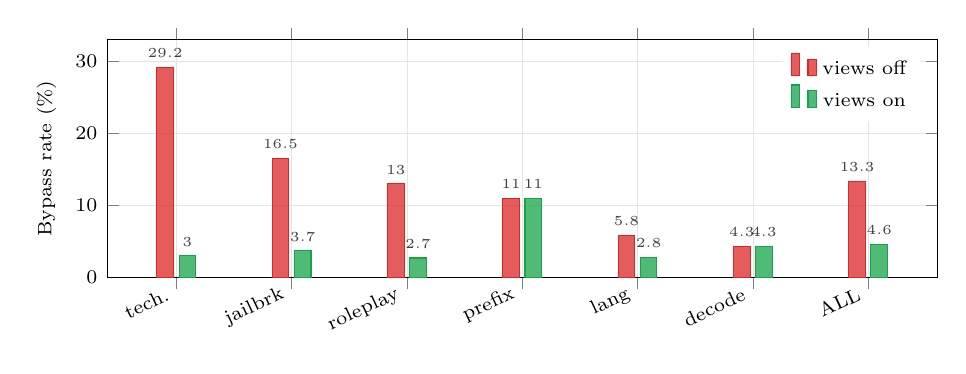
\begin{tikzpicture}
\begin{axis}[
  width=\columnwidth, height=4.6cm,
  ybar, bar width=6pt,
  ylabel={Bypass rate (\%)},
  symbolic x coords={tech.,jailbrk,roleplay,prefix,lang,decode,ALL},
  xtick=data, x tick label style={font=\scriptsize,rotate=25,anchor=east},
  ymin=0,ymax=33,
  grid=major, grid style={line width=.2pt,draw=gray!20},
  tick label style={font=\scriptsize}, label style={font=\scriptsize},
  legend style={font=\scriptsize,at={(0.98,0.97)},anchor=north east,draw=none},
  nodes near coords, every node near coord/.append style={font=\tiny},
]
\addplot[draw=cBad,fill=cBad,fill opacity=.75] coordinates {
(tech.,29.2)(jailbrk,16.5)(roleplay,13.0)(prefix,11.0)(lang,5.8)(decode,4.3)(ALL,13.3)};
\addlegendentry{views off}
\addplot[draw=cGood,fill=cGood,fill opacity=.75] coordinates {
(tech.,3.0)(jailbrk,3.7)(roleplay,2.7)(prefix,11.0)(lang,2.8)(decode,4.3)(ALL,4.6)};
\addlegendentry{views on}
\end{axis}
\end{tikzpicture}
\caption{Guard-bypass rate over 3{,}600 paired variants, with and without
leading-clause payload views. The intervention targets framing attacks and
leaves the two it does not address, \texttt{prefix\_rewrite} and
\texttt{decoding\_manipulation}, exactly unchanged.}
\label{abr:fig:views}
\end{figure}

\setcounter{table}{20}
\begin{table}[!htbp]
\caption{HarmBench attack pass, 200 requests $\times$ 6 attacks $\times$ 3
variants, by checkpoint. Intervals are seed-clustered.}
\label{abr:tab:attack}
\centering
\scriptsize
\begin{tabular}{@{}lccc@{}}
\toprule
Checkpoint & Bypassed / variants & Rate & 95\% CI \\
\midrule
Historical & 165 / 3600 & \best{4.6}\% & [2.5, 6.8] \\
Seed 43    & 180 / 3600 & 5.0\% & [2.8, 7.4] \\
Seed 42    & 226 / 3600 & 6.3\% & [3.9, 9.1] \\
Seed 44    & 282 / 3600 & 7.8\% & [5.2, 10.9] \\
\bottomrule
\end{tabular}
\end{table}

\setcounter{table}{21}
\begin{table}[!htbp]
\caption{Expected calibration error of the graded harm scores, ten
equal-width bins, with 95\% bootstrap intervals over prompts. In distribution:
the pool test split for Layer~1 ($n=1912$, balanced) and the 300 pool-validation
prompts of the tuning run for the judges. Final test set: the 3{,}089 primary
prompts, pooled over single-class sources (1{,}874 safe, 1{,}215 harmful), so
these values are conditional on that mixture. Post hoc, from stored scores.}
\label{abr:tab:ece}
\centering
\scriptsize
\setlength{\tabcolsep}{4pt}
\begin{tabular}{@{}lcc@{}}
\toprule
Score & In distribution & Final test set \\
\midrule
Layer 1, configured checkpoint & 0.013 [0.008, 0.021] & 0.204 [0.191, 0.221] \\
Layer 1, retrained s42 / s43 / s44 & --- & 0.252 / 0.226 / 0.222 \\
Judge, Qwen2.5-3B & 0.191 [0.153, 0.242] & 0.172 [0.159, 0.186] \\
Judge, Llama-3.2-3B\posthoc & 0.102 [0.072, 0.141] & 0.129 [0.117, 0.141] \\
Granite Guardian & --- & 0.211 [0.199, 0.225] \\
Llama Guard & --- & 0.155 [0.143, 0.169] \\
ShieldGemma\posthoc & --- & 0.167 [0.153, 0.182] \\
\bottomrule
\end{tabular}
\end{table}

\setcounter{table}{22}
\begin{table}[!htbp]
\caption{The identical training recipe under three seeds, scored on the final
test set. Ranges are observed spreads, not confidence intervals.}
\label{abr:tab:seeds}
\centering
\scriptsize
\begin{tabular}{@{}lcccc@{}}
\toprule
Source & Historical & s42 & s43 & s44 \\
\midrule
CatQA (harmful allowed)     & 19.2 & 34.8 & 22.3 & 35.7 \\
DNA core (harmful allowed)  & 23.9 & 25.8 & 23.4 & 23.6 \\
PHTest (safe blocked)       & 42.8 & 45.9 & 46.3 & 42.2 \\
No Robots (safe blocked)    & 12.7 & 14.1 & 15.3 & 10.5 \\
\midrule
Pooled AUROC                & 0.811 & 0.751 & 0.773 & 0.777 \\
\bottomrule
\end{tabular}
\end{table}

\setcounter{table}{23}
\begin{table}[!htbp]
\caption{The Layer-2 slot under two models, against the cascade that contains
it. Percent; harmful sources report harmful allowed, safe sources safe blocked;
lower is better throughout. Both Llama arms are post hoc. Do-Not-Answer
``other'' is excluded as secondary, as in Table~\ref{tab:rates}; it is the
source on which the substitute trails the cascade most, at \SI{69.0}{\percent}
against \SI{48.9}{\percent}.}
\label{abr:tab:judgeswap}
\centering
\scriptsize
\setlength{\tabcolsep}{4pt}
\begin{tabular}{@{}lcccc@{}}
\toprule
& & \multicolumn{3}{c}{Layer-2 slot, judged alone} \\
\cmidrule(lr){3-5}
Source & Cascade & Qwen2.5 & Llama v1\posthoc & Llama v2\posthoc \\
\midrule
SimpleSafetyTests  & 5.1 & 2.0 & \best{0.0} & \best{0.0} \\
CatQA              & 19.2 & 2.4 & \best{0.9} & 1.8 \\
Do-Not-Answer core & \best{23.9} & 32.6 & \best{23.9} & 32.5 \\
\midrule
CoCoNot contrast   & \best{6.3} & 20.4 & 21.7 & 13.5 \\
PHTest harmless    & 42.8 & 29.6 & 25.7 & \best{17.2} \\
No Robots          & 12.7 & 7.1 & 5.4 & \best{2.4} \\
\bottomrule
\end{tabular}
\end{table}

\end{document}
